\begin{frame}{Eigenschaften Embedded System\hcite{embeddedSpecials}}
	\pause
	\begin{multicols}{2}
		\begin{itemize}
			\item Kosten
			\item Grösse
			\item Energie
			\item Zuverlässigkeit
			\item Sicherheit
			\item Langlebigkeit
			\item Echtzeit
		\end{itemize}
	\end{multicols}
\end{frame}

\begin{frame}{Definition Embedded System}
	Der Ausdruck embedded system bezeichnet einen Computer, der in einem technischen Kontext eingebettet ist. \hcite{wikiEmbedded}
	\begin{flushright}
		Nach Wikipedia
	\end{flushright}
\end{frame}

\begin{frame}{Embedded Systeme}
	\footnotesize{
	\begin{multicols}{2}
				\only<handout>{Digitales Multimeter}
				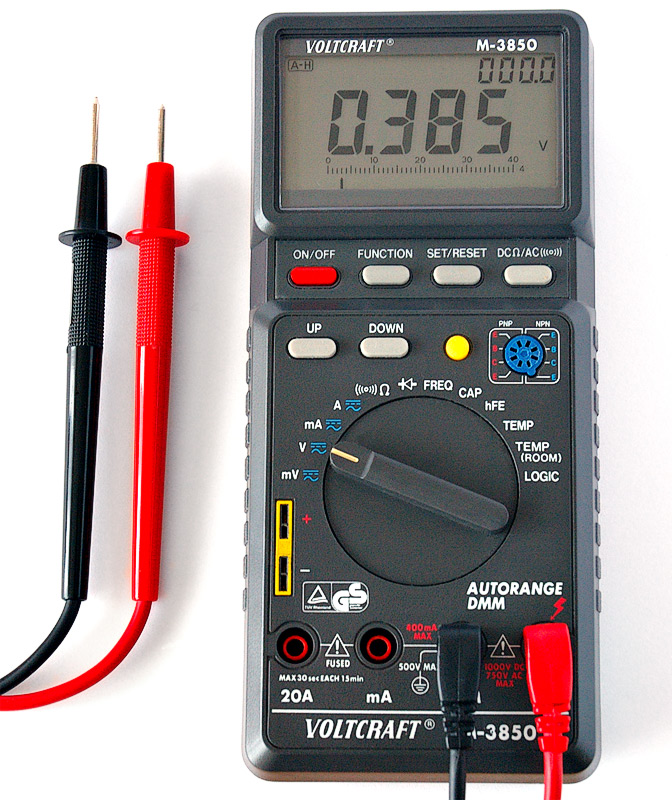
\includegraphics[height=4cm]{res/Digital_Multimeter_Aka.jpg}\hcite{multimeter}
				\only<handout>{
					\begin{itemize}
						\item Sensor produziert ~20 B/sec
						\item Reduzierung auf ~2 B/sec
						\item Verarbeitung auf internem uC
					\end{itemize}
				}
				\pagebreak
				\only<handout>{ATLAS/LHC/CERN}
				\visible<2->{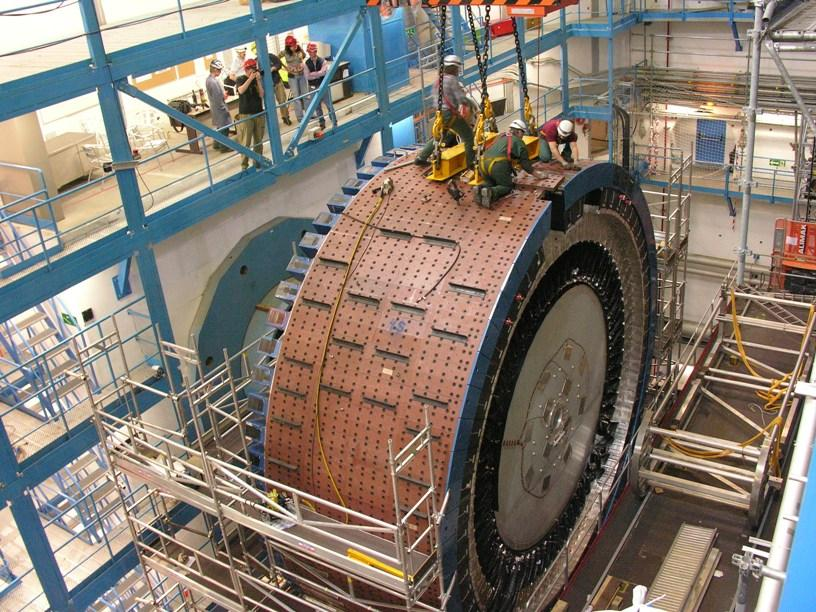
\includegraphics[height=4cm]{res/ATLAS_Tile_Calorimeter}\hcite{tileCalorimeter}}
				\only<handout>{
					\begin{itemize}
						\item Sensor produziert 1 PiB/sec
						\item Reduzierung auf ~100 MiB/sec \hcite{wikiAtlas}
						\item Verarbeitung auf eigenen 20'000 Server und Grid \hcite{wikiCernServer}
					\end{itemize}
				}
	\end{multicols}
	}
\end{frame}

\begin{frame}{Typisches GNU/Linux Embedded System}
	\begin{center}
		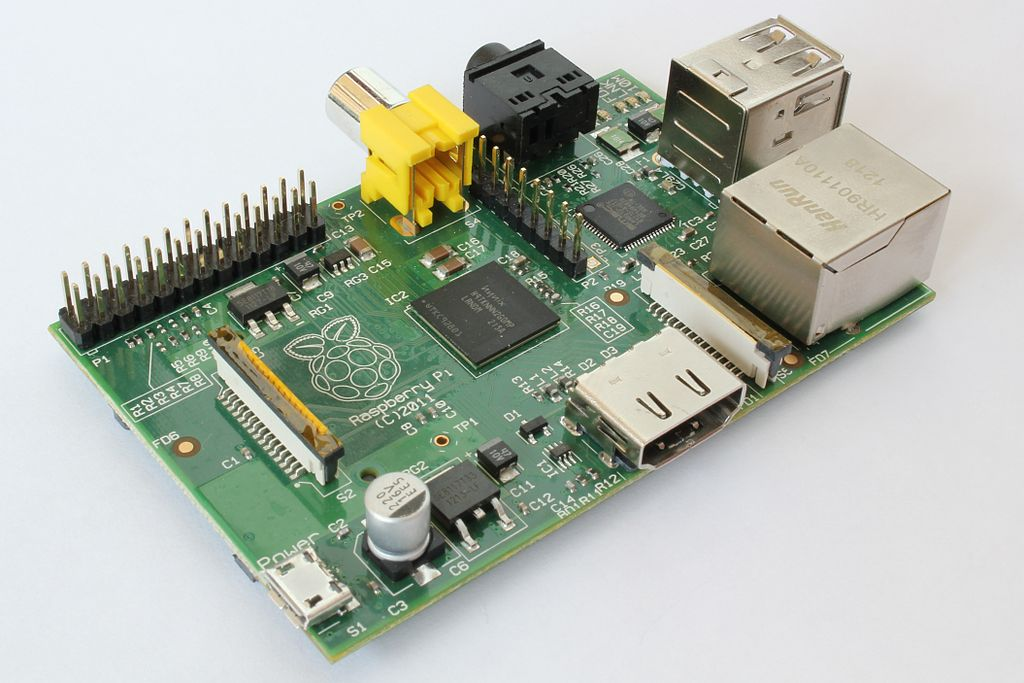
\includegraphics[width=5cm]{res/RaspberryPi.jpg}\hcite{raspberryPi}
		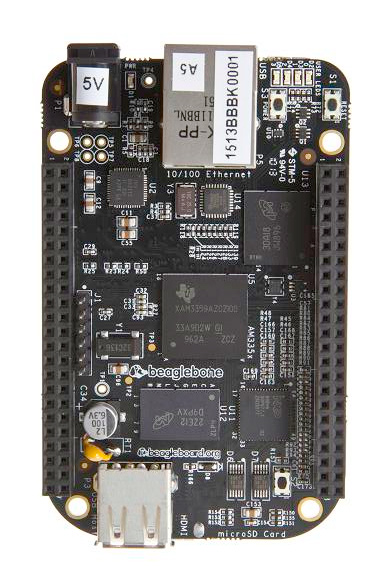
\includegraphics[width=3.5cm]{res/Beaglebone_Black.jpg}\hcite{beagleboneBlack}
	\end{center}
\end{frame}

\begin{frame}{Echtzeit}
	\begin{center}
		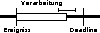
\includegraphics[width=8cm]{res/echtzeit.pdf}
	\end{center}
	\only<handout>{
		\begin{itemize}
			\item Bearbeitung ist nach einer bestimmten Zeit nach dem auftreten eines Ereignisses abgeschlossen.
			\item bei weicher Echtzeit ist dieses Verhalten wünschenswert (Video Wiedergabe)
			\item Echtzeit ist oft nicht nötig
			\item Linux ist nicht Echtzeit-Fähig
			\item Lösung ist separater uC, im SOC oder dediziertem Chip
		\end{itemize}
	}
\end{frame}
